
\chapter{Introduction}

\section{Background}
Human motion generation using skeleton-based 3D motion data has gained significant attention from researchers across various fields, including computer graphics, robotics, human-computer interaction (HCI), and computer vision. The primary objective of human motion generation is to develop models that are capable of synthesizing realistic, natural, and diverse human motions. These synthesized motions find applications across a broad spectrum, including digital film production, games, augmented/virtual reality (AR/VR), sports analysis, smart healthcare, human-robot interaction (HRI), and the creation of intelligent virtual avatars (IVAs).

Typically, a human motion generation task is conditioned on various factors, such as text \cite{dummy}, audio \cite{dummy}, scene \cite{dummy}, or another motion sequence \cite{dummy}. In recent years, there has been a significant surge in the development of diverse generative methods, primarily driven by advancements in deep learning \cite{dummy}. These approaches include Autoregressive models \cite{dummy}, Variational Autoencoders (VAE) \cite{dummy}, Normalizing Flows \cite{dummy}, Generative Adversarial Networks (GAN) \cite{dummy}, and Denoising Diffusion Probabilistic Models (DDPM) \cite{dummy}. These methodologies have demonstrated their effectiveness in various domains such as text \cite{dummy}, \cite{dummy}, imagery \cite{dummy}, video \cite{dummy}, and 3D objects \cite{dummy}. Additionally, significant progress in human motion modelling \cite{dummy} has enabled the extraction of human motion from videos \cite{dummy}, as well as the creation of extensive human motion datasets \cite{dummy}. Consequently, there has been growing interest within the research community in data-driven approaches for human motion generation in recent times.

Human motion generation presents several challenges ...


\begin{figure}[t]	
	\centering
	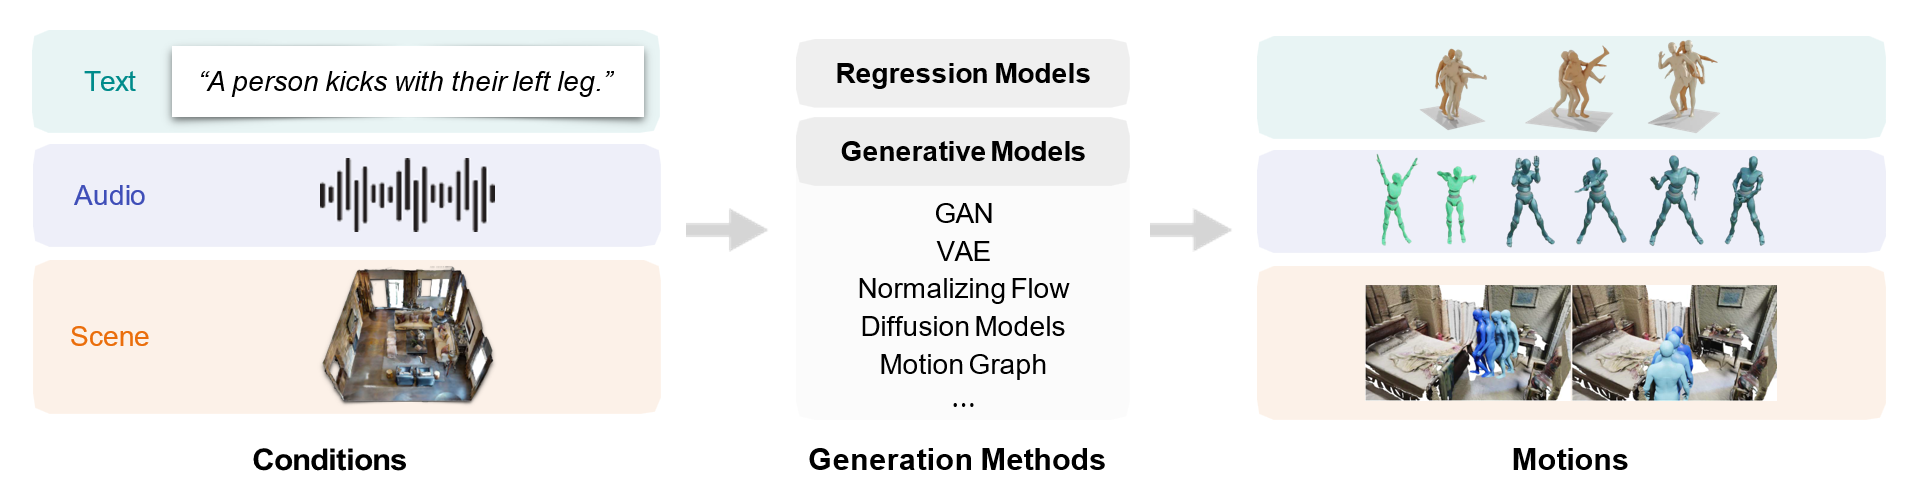
\includegraphics[width=1\textwidth]{figures/chapter1/fig_hmg_gan}
	\caption{An overview of typical human motion generation approaches. Example images adapted from \cite{dummy}.}
	\label{fig_hmg_gan}
\end{figure}
 
\section{Motivation}
Generating accurate 3D motions is a hot topic in the field of computer vision. Researchers are proposing various methods to generate human motions, such as predicting motions based on historical sequences, generating motions for a particular action class, and creating motions that follow a trajectory or a song. These methods aim to produce increasingly realistic and complex motions. There are numerous potential applications for these generative methods in various areas, which has sparked the interest of researchers.\\

\subsection{Human-Robot Interaction (HRI)}

\noindent
Safe and Efficient Collaboration: The utilization of human motion generation in training robots to predict human movements results in enhanced collaboration efficiency and safety within shared work environments. The simulation of various human actions enables robots to adapt their behavior and movements accordingly, thereby reducing the occurrence of collisions or accidents.

\noindent
Enhanced Robot Configuration: Through the generation of diverse and intricate human motions, scholars can assess and enhance the design of robots. This process involves examining a robot's capacity to maneuver ...


\section{Research Gaps in Existing Studies}
Despite the progress made in human motion generation, there exist significant gaps and opportunities for further research and development. We identify the following limitations and lack of research in the domain:\\

\noindent
\textbf{Bridging action semantics and raw motion}: The fundamental challenge lies in establishing a meaningful connection between the raw motion space and the action semantic space \cite{dummy}. Conventionally, raw motion is represented as a sequence of 3D poses \cite{dummy} or SMPL model parameters \cite{dummy}, while action semantics are characterized by action categories or textual descriptions in natural language. Existing approaches for human motion generation often struggle to produce realistic motion sequences due to significant gap in mapping from action semantic text to raw motion pose sequence. Creating stronger connection between action semantics and raw motion with the aid of intermediate motion representations can make human motion understand more intuitive and improve the performance of underlying motion tasks. \\

\noindent
\textbf{Human reaction motion generation}: Existing research mostly focus on generating human motion for a single character, while neglecting the motion sequences where interaction of two persons are involved. There is an opportunity for creating methods that generate reactive motion of one character when the action sequence of other is given.\\

\noindent
\textbf{Human interaction generation}: Existing methods recognize and label the human interactions, but there is a lack of research pertaining to generation of motion sequences for interacting characters.\\

\noindent
\textbf{Accurate 3D human pose estimation}: In human-agent interactions, 3D human pose estimation is fundamental. The quality of extracted 3D skeletons for human motion is directly proportional to the accuracy of motion models. Despite recent progress in 3D human pose estimation methods, practical applications often encounter challenges, particularly when dealing with complex poses commonly found in human motion sequences. Proposing an accurate 3DHPE method dealing with complex poses can benefit more accurate human motion generation models.



\begin{figure}[!t]	
	\centering
	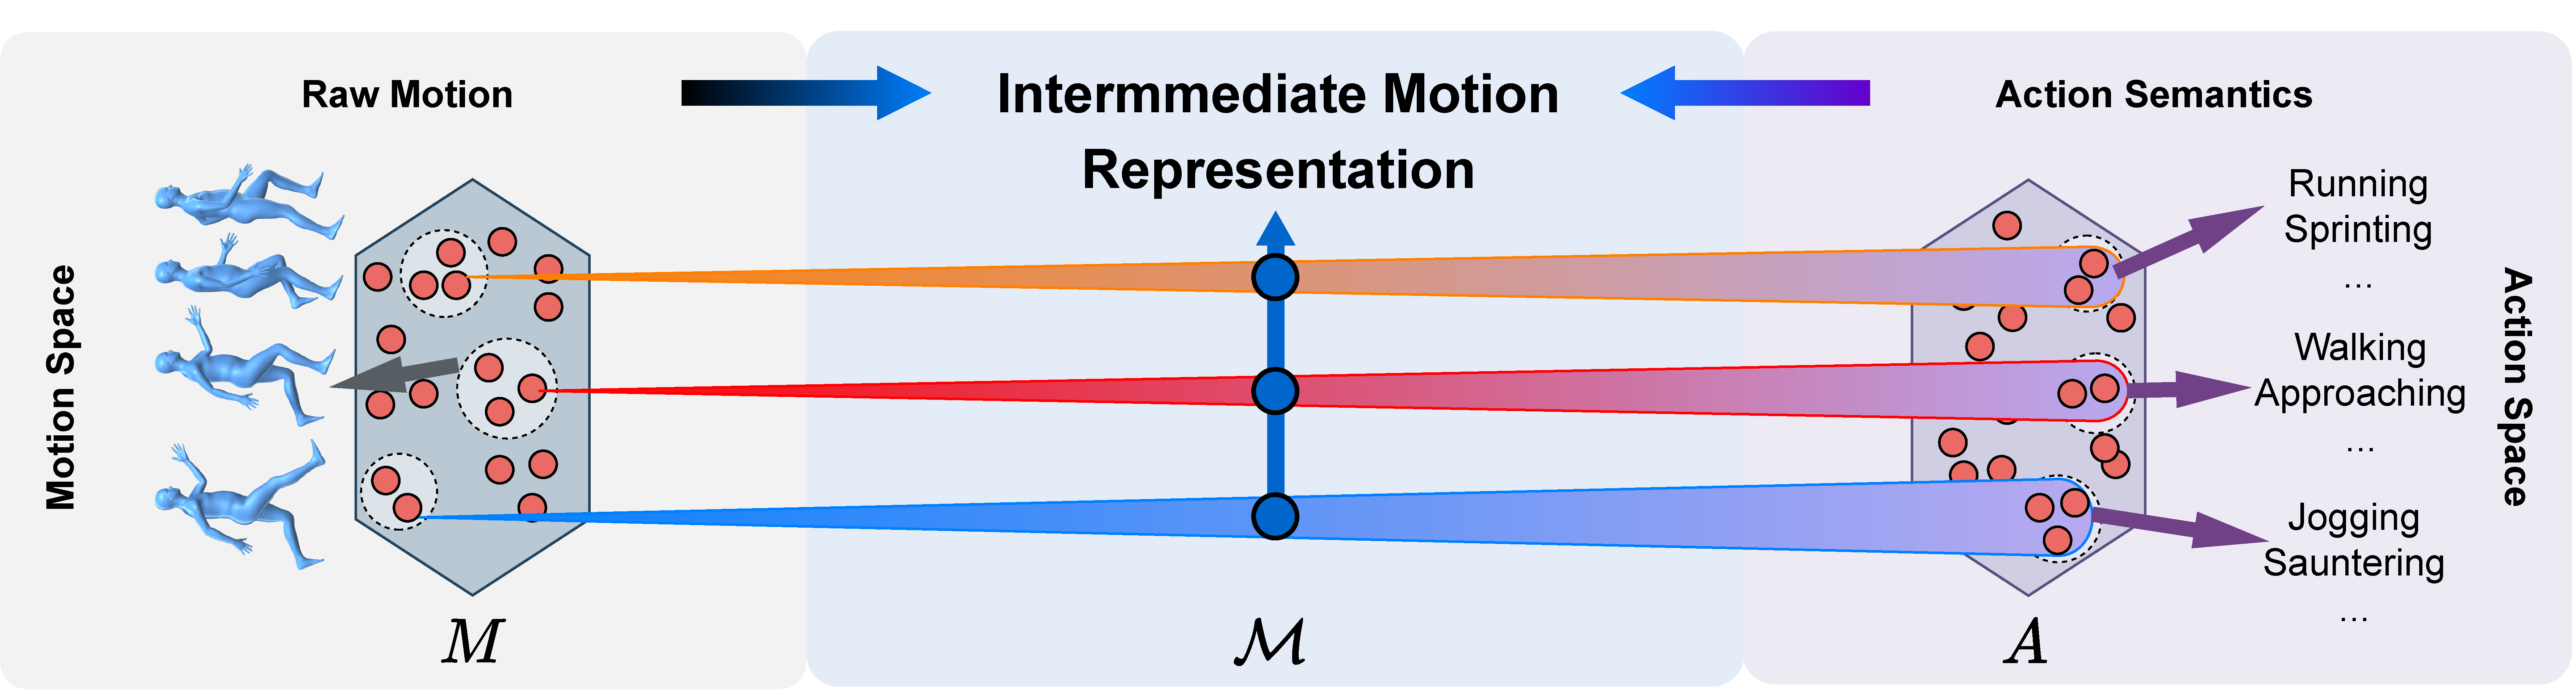
\includegraphics[width=1\textwidth]{figures/chapter1/fig_problem_statement_1}
	\caption{Visualizing semantic gap between action semantics and raw motion.}
	\label{fig_problem_statement_1}
\end{figure}

\begin{figure}[!t]	
	\centering
	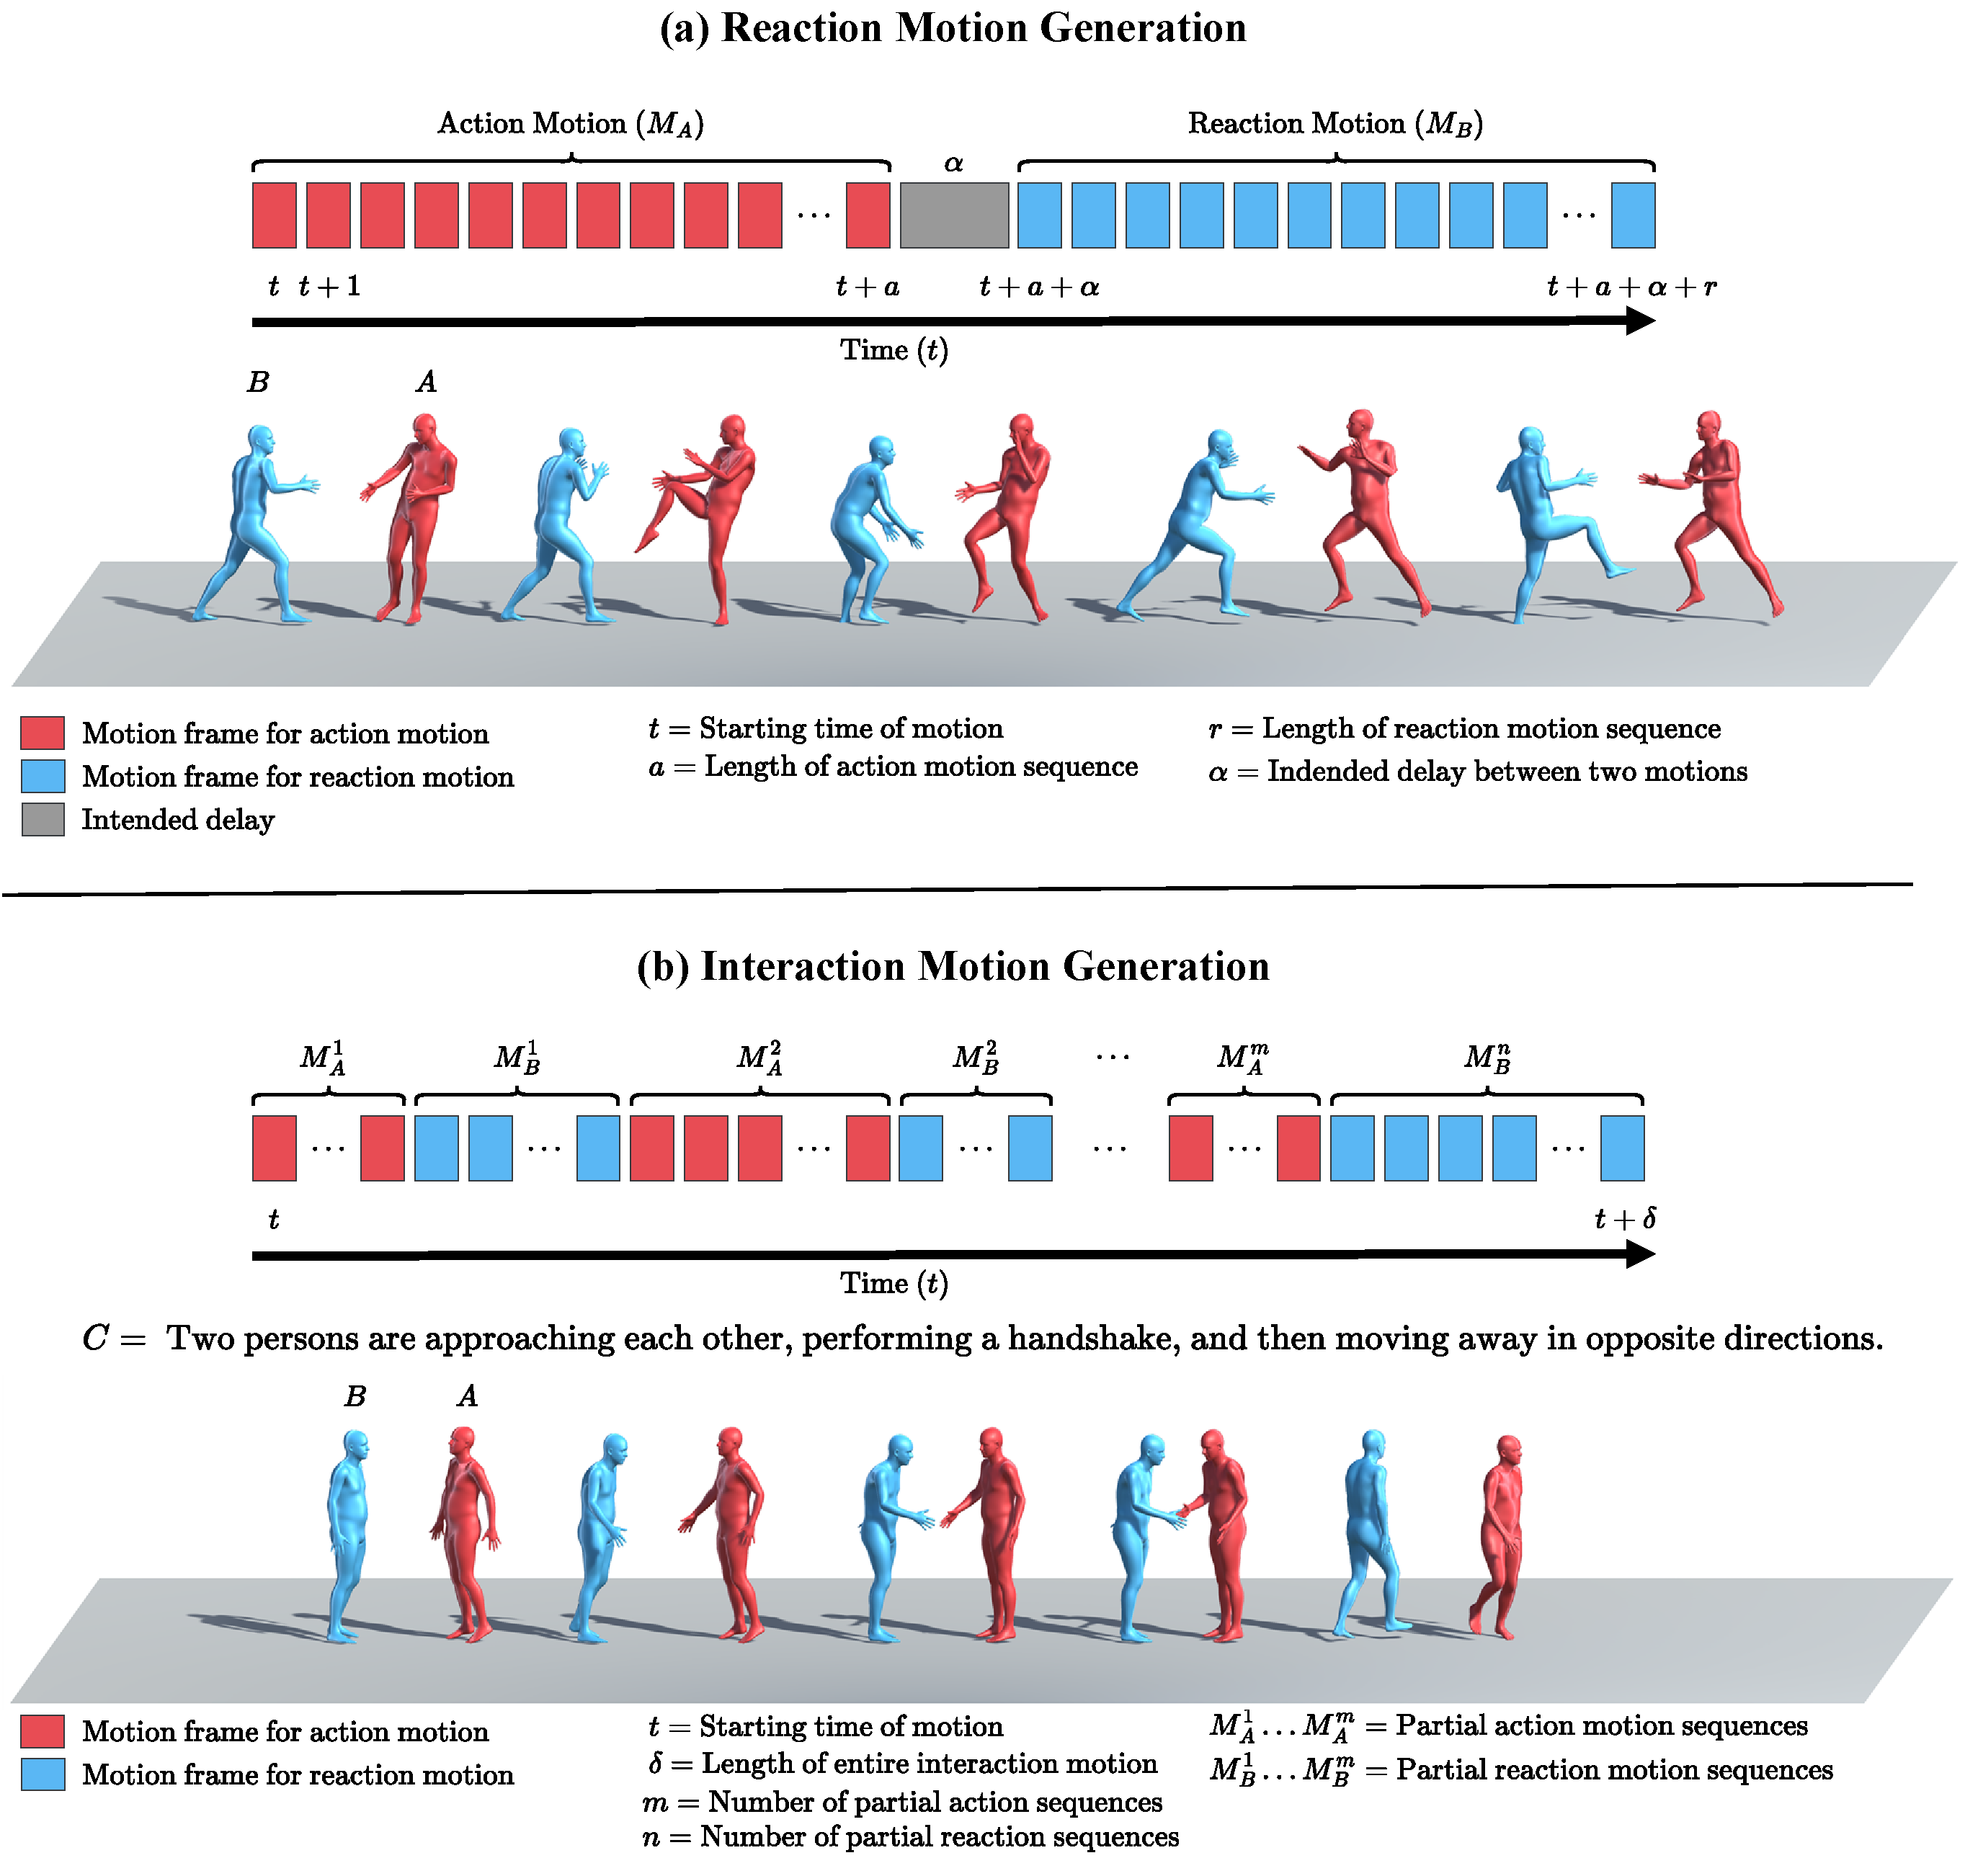
\includegraphics[width=1\textwidth]{figures/chapter1/fig_problem_statement}
	\caption{Illustration and mathematical symbols for various human motion generation process. The virtual character in red (Character A) represents the actor performing an action sequence. The character in blue (Character B) represents the actor performing a reaction sequence. (a) The illustration for reaction generation, when action motion sequence is given. (b) The illustration for interaction generation, given the conditioned signal $C$.}
	\label{fig_problem_statement}
\end{figure}




\section{Problem Formulation}
Consider the reaction motion generation concept illustrated in Fig.\ref{fig_problem_statement} (a) and interaction motion generation shown in Fig. \ref{fig_problem_statement} (b), we define following problem statements for this thesis:

\begin{enumerate}
	\item Developing an effective methodology to bridge action semantics $A$ and raw motion $M$ by generating an stronger intermediate motion representation $\mathcal{M}$. The intermediate representation is devised such that the mapping $A\mapsto \mathcal{M} \mapsto M$, ultimately leads to motion generation characterized by improved precision, diversity, multi-modality, and accuracy across various motion generation tasks.
	\item Given a action motion sequence $M_B$ of virtual character $B$, develop a motion generator network to generate corresponding reaction motion sequence $M_A$ of character $A$, where $M_A \in \mathbb{R}^{T \times J \times 3}$ and $M_B \in \mathbb{R}^{T \times J \times 3}$ are the sequences of skeleton poses with $J$ number of joints and $T$ number of frames.
	\item Developing a motion generation network to simultaneously generate partial interactive motion sequences ${M_A^1, \dots, M_A^m}$ and ${M_B^1, \dots, M_B^n}$ for character $A$ and character $B$, respectively, given a textual context $C$ in a dyadic interaction scenario. Where each partial motion $M_A^M \in \mathbb{R}^{T \times J \times 3}$ and $M_B^N \in \mathbb{R}^{T \times J \times 3}$ are the sequences of skeleton poses with $J$ number of joints and $T$ number of frames (while $T$ may be variable for each sequence).
	\item Given a monocular RGB image $I$, develop an pose estimation network to output a 3D human pose $P$, where $P \in \mathbb{R}^{J \times 3}$ and $J$ is the number of skeleton joints.
\end{enumerate}


\section{Research Questions}

The study identifies and tries to answer the following research questions:

RQ1: How can intermediate motion representations effectively bridge the gap between action semantics and raw motion, improving the realism of generated motion sequences?

RQ2: What novel methods can be devised to generate reactive motion sequences for a character in response to the action sequence of another character?

RQ3: How can motion generation networks be designed and trained to accurately produce motion sequences for interacting characters in dyadic interactions?

RQ4: What advancements can be made in 3D human pose estimation to enhance the accuracy of extracted poses, particularly in dealing with complex poses commonly found in human motion sequences?

RQ5: How can a comprehensive framework integrating improved pose estimation, action-motion semantic comprehension, reaction motion modeling, and interactive motion modeling be designed and implemented to improve the naturalness and realism of generated human motion sequences?


\section{Research Aim and Objectives}
This aim of the study is to proposes a comprehensive framework to facilitate the generation of human motion sequences, incorporating coarse-to-fine pose estimation, action semantic comprehension, reaction motion modeling, and interactive motion modeling to improve the realism and naturalness of the generated motion sequences. The objective of the study are:

\begin{enumerate}
	\item To identify and propose intermediate motion representation to effectively bridge action semantics and raw motion.
	\item Designing and developing a network to generate the reaction motion sequence given the action motion sequence.
	\item Designing and developing a network to generate interaction motion sequence in dyadic interactions.
	\item Designing and developing an accurate 3D human pose estimation network to yield a 3D human pose given a monocular image. 
\end{enumerate}


\section{Significance of the study}
This research holds significant implications for numerous applications, including entertainment, education, healthcare, and human-computer ...



\section{Contributions of the Study}
This thesis makes several contributions to the field of human motion synthesis, including novel algorithms, methodologies, and insights that address key challenges and advance the state-of-the-art...

\section{Thesis Organization}
\noindent
Chapter 2: This chapter provides a comprehensive ...

\noindent
Chapter 3: This chapter introduces a novel methodology ...

\noindent
Chapter 4: This chapter presents a novel approach ...

\noindent
Chapter 5: This chapter employs anthropometric constraints ...



\begin{figure*}[!t]
	\centering
	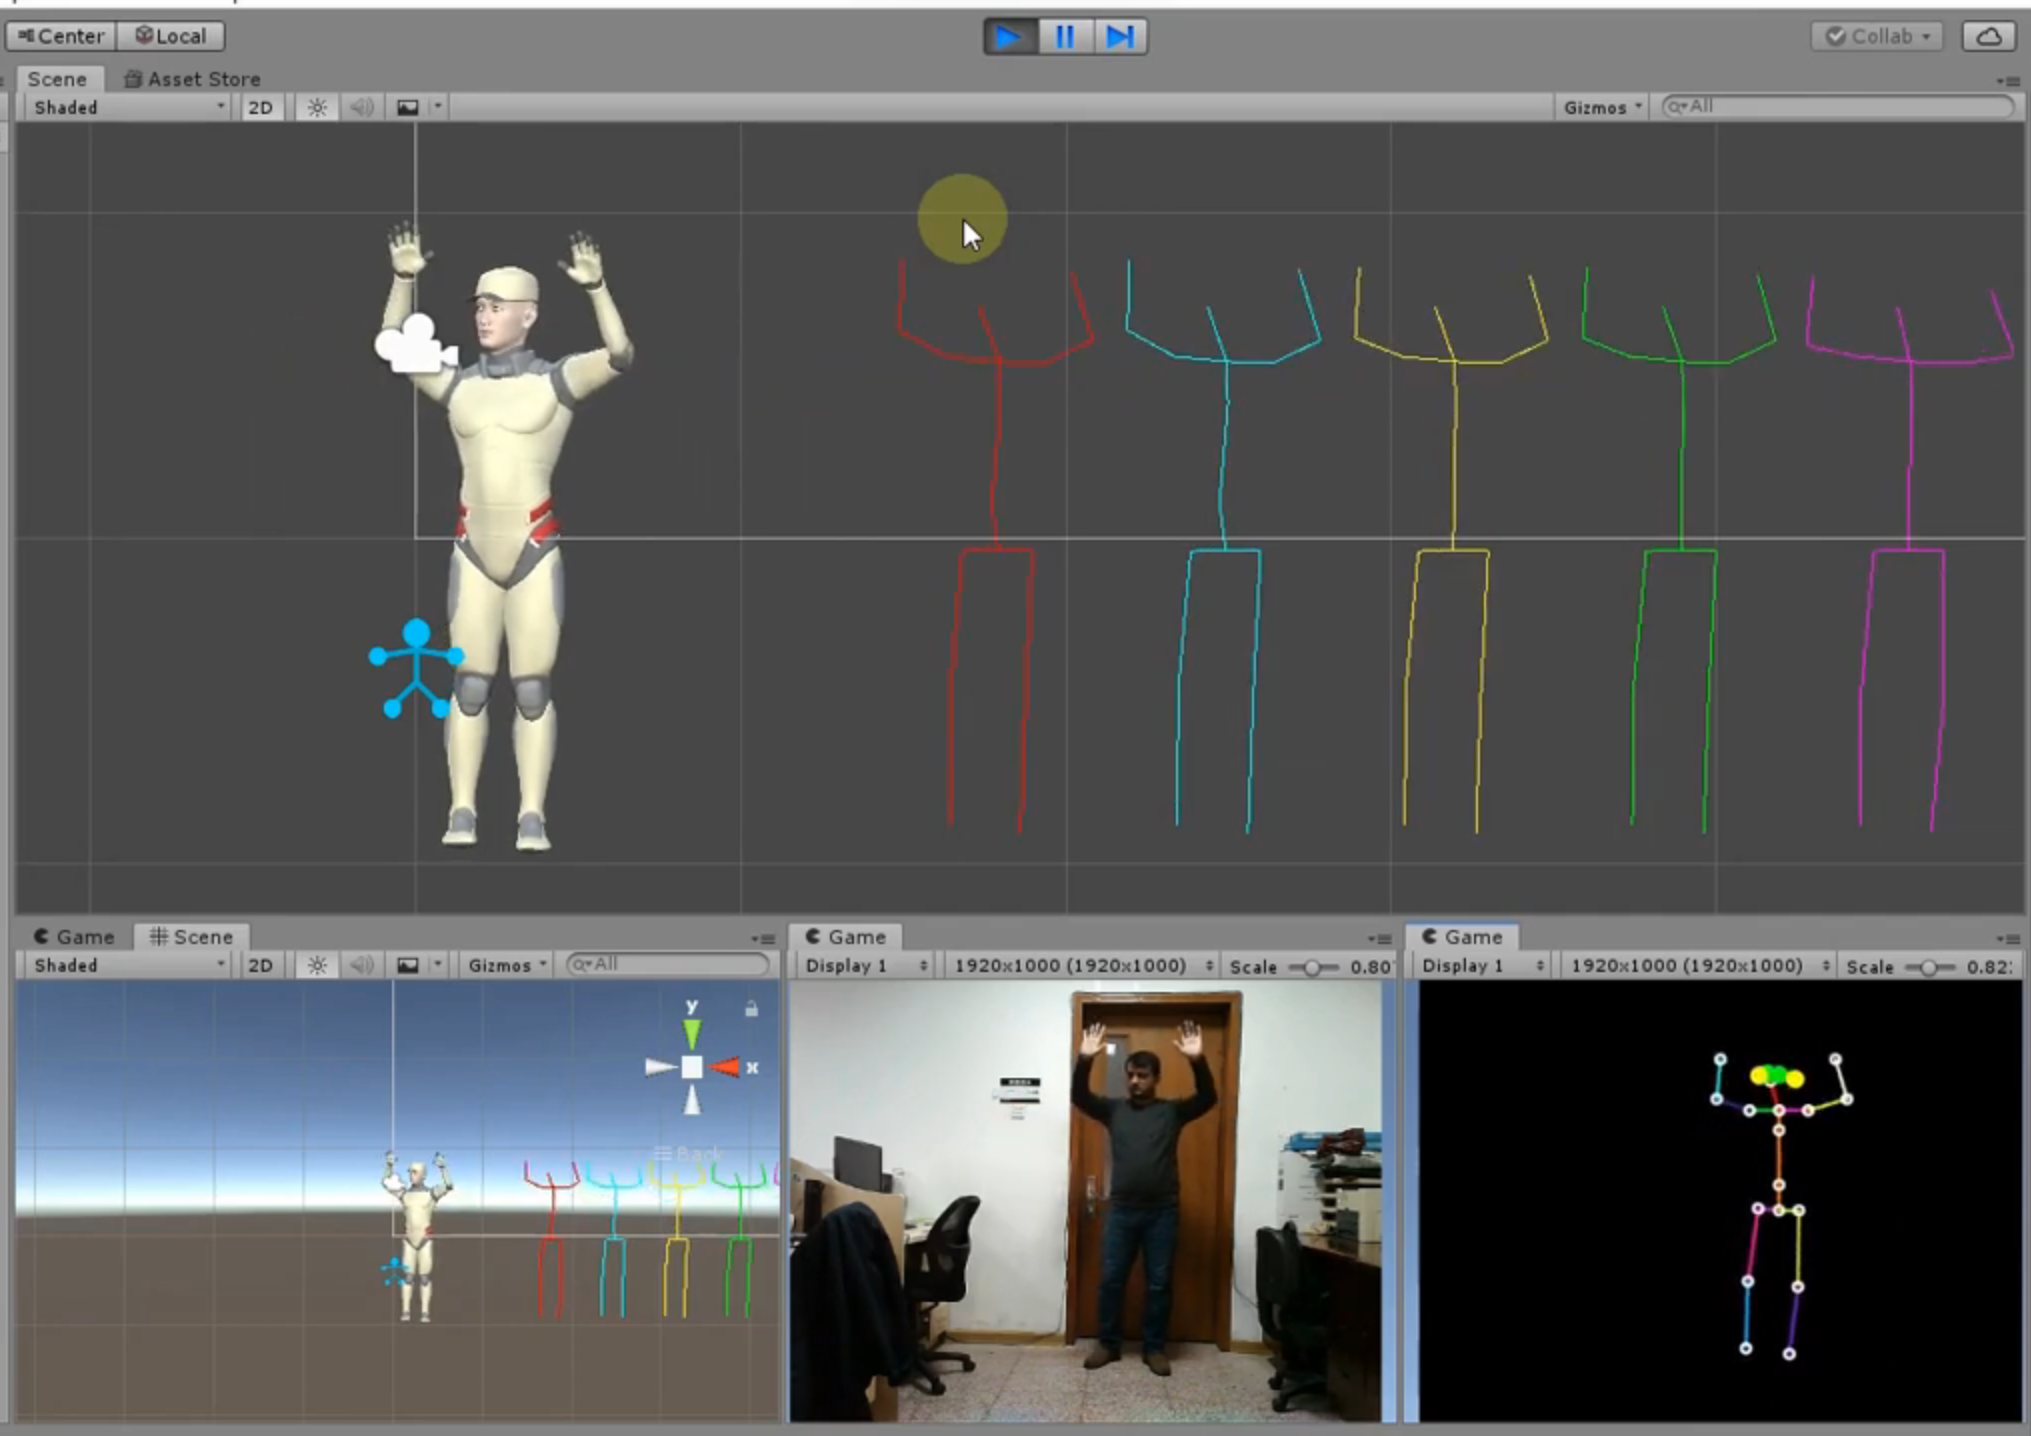
\includegraphics[width=1\textwidth]{figures/chapter1/fig_human_avatar_2}
	\caption{Human avatar interaction in virtual reality.}
	\label{fig_gap}
\end{figure*}




